% =============================================================================
% P3D -- Privacidade 2: pôster (PT-BR), versão style2
% Estilo do pôster da P2A (_grupo/P2A/mainV3.tex): a0poster A1 retrato, marca da UnB,
% título em versalete verde, duas colunas com títulos azuis numerados, sem caixas.
% Figuras esperadas em out/: FigP1_PT.pdf, FigP3_PT.pdf (compiladas de figuras/).
% O mapa de calor (Figura 2) é uma tabela colorida escrita neste arquivo.
% Marca da UnB: figuras/marca_unb.png. Conteúdo igual ao do pôster P3D_Privacidade2_Poster_PT.tex.
% =============================================================================
\documentclass[a1,portrait]{a0poster}
\usepackage[brazil]{babel}
\usepackage[utf8]{inputenc}
\usepackage[absolute]{textpos}
\usepackage{graphicx}
\usepackage{color}
\usepackage[table]{xcolor}
\usepackage{amsmath,amssymb}
\usepackage{booktabs}

\definecolor{DarkBlue}{rgb}{0.1,0.1,0.5}
\definecolor{Red}{rgb}{0.9,0.0,0.1}
\definecolor{DarkGreen}{rgb}{0.10,0.50,0.10}
\definecolor{exLine}{RGB}{23,54,93}

\let\Textsize\normalsize
\def\LHead#1{\noindent{\LARGE\color{DarkBlue} #1}\smallskip}
\def\Subhead#1{\noindent{\large\color{DarkBlue} #1}}
\newcommand{\quiteHuge}{\fontsize{55}{70}\selectfont}
\def\Title#1{\begin{center}\noindent{\quiteHuge\color{DarkGreen}#1}\end{center}}

\TPGrid[40mm,40mm]{23}{12}

\parindent=0pt
\parskip=0.5\baselineskip

\begin{document}
\large

\begin{textblock}{23}(0,0)
\centering

\includegraphics[width=18cm]{figuras/marca_unb.png}
\end{textblock}

\begin{textblock}{23}(0,0.5)
\Title{\textsc{PMBOK 8 em uma página: princípios, processos e adaptação sob medida}}
\end{textblock}

\begin{textblock}{23}(0,1.45)
\begin{center}
  \parbox{0.8\textwidth}{
    \small
    \begin{center}
    \textbf{Autores:} Filipe Alves de Sousa e Membros do Grupo Colégio Reciclagem 1\\
    \textbf{Disciplina:} Gestão de Projetos de TI (GPTI) -- PPCA/CIC/UnB\\
    \textbf{Entrega:} P3D | \textbf{Código:} 3p2 / 3R31
    \end{center}
  }
\end{center}
\end{textblock}

% ------------------------------- COLUNA ESQUERDA ------------------------------
\begin{textblock}{11}(0,2.3)

\LHead{1. Princípios e adaptação}

Princípios orientam decisões; domínios e áreas de foco organizam o trabalho; \textit{tailoring} ajusta sua aplicação [4].

\begin{figure}[h!]
\centering
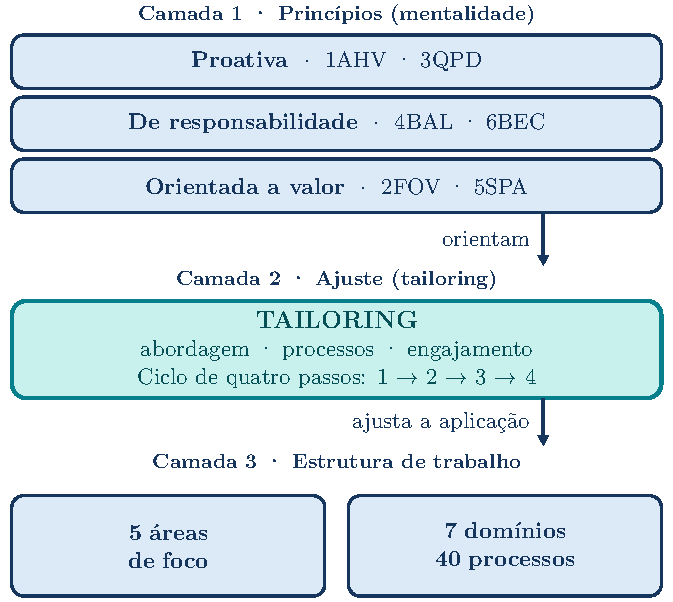
\includegraphics[width=\linewidth]{out/FigP1_PT.pdf}
\caption{Princípios e adaptação.}
\end{figure}

\textbf{Cinco operações sobre processos:} adicionar $\cdot$ modificar $\cdot$ remover $\cdot$ combinar $\cdot$ alinhar. \textbf{Três objetos da adaptação:} ciclo de vida e abordagem de desenvolvimento $\cdot$ processos $\cdot$ engajamento [4].

\vspace{0.3cm}
\LHead{2. Mapa dos 40 processos}

{\normalsize
\setlength{\tabcolsep}{4pt}
\renewcommand{\arraystretch}{1.3}
\noindent\begin{tabular*}{\linewidth}{@{\extracolsep{\fill}}lrrrrrr}
\hline
\textbf{Domínio} & \textbf{IN} & \textbf{PL} & \textbf{EX} & \textbf{MC} & \textbf{CL} & \textbf{Total}\\
\hline
Governança & \cellcolor{exLine!9}1 & \cellcolor{exLine!18}2 & \cellcolor{exLine!27}3 & \cellcolor{exLine!18}2 & \cellcolor{exLine!9}1 & 9\\
Escopo & 0 & \cellcolor{exLine!36}4 & 0 & \cellcolor{exLine!18}2 & 0 & 6\\
Cronograma & 0 & \cellcolor{exLine!18}2 & 0 & \cellcolor{exLine!9}1 & 0 & 3\\
Finanças & 0 & \cellcolor{exLine!27}3 & 0 & \cellcolor{exLine!9}1 & 0 & 4\\
Partes Interessadas & \cellcolor{exLine!9}1 & \cellcolor{exLine!18}2 & \cellcolor{exLine!18}2 & \cellcolor{exLine!18}2 & 0 & 7\\
Recursos & 0 & \cellcolor{exLine!18}2 & \cellcolor{exLine!18}2 & \cellcolor{exLine!9}1 & 0 & 5\\
Riscos & 0 & \cellcolor{exLine!36}4 & \cellcolor{exLine!9}1 & \cellcolor{exLine!9}1 & 0 & 6\\
\hline
\textbf{Total} & \textbf{2} & \textbf{19} & \textbf{8} & \textbf{10} & \textbf{1} & \textbf{40}\\
\hline
\end{tabular*}\par}

\vspace{0.2cm}
{\small \textbf{Legenda:} IN Iniciação $\cdot$ PL Planejamento $\cdot$ EX Execução $\cdot$ MC Monitoramento e Controle $\cdot$ CL Encerramento. Contagem de processos $\neq$ duração ou importância de uma área. \textit{Identify Stakeholders} está em Iniciação (Figura 2-32 do \textit{Guide}).}

\end{textblock}

% ------------------------------- COLUNA DIREITA -------------------------------
\begin{textblock}{11}(12,2.3)

\LHead{3. Quatro concentrações dos domínios}

\begin{figure}[h!]
\centering
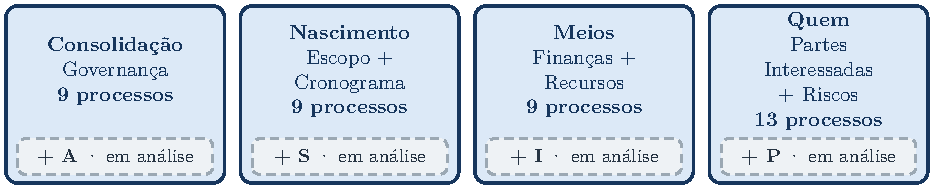
\includegraphics[width=\linewidth]{out/FigP3_PT.pdf}
\caption{Quatro concentrações dos domínios.}
\end{figure}

\textbf{Aviso de leitura:} as quatro concentrações e as etiquetas A, S, I e P são \textbf{agrupamento analítico deste trabalho}; os sete domínios e seus 40 processos são do PMBOK 8 [4].

\vspace{0.3cm}
\LHead{4. Como usar a síntese}

Escolha uma abordagem inicial, adapte-a à organização e ao projeto e melhore-a continuamente [4]. O mapa localiza os 40 processos, sem impor uma sequência única; a contagem por área não indica duração nem importância. O PMBOK 8 não descreve gêmeos digitais. Estudos sobre abordagens híbridas [3, 5] ajudam a contextualizar decisões de adaptação.

\vspace{0.3cm}
\LHead{5. Referências principais}

{\normalsize
[3] NOLL, J.; BEECHAM, S. How agile is hybrid agile? An analysis of the HELENA data. \textbf{PROFES 2019}, LNCS v. 11915, p. 341--349, 2019.

[4] PMI. \textbf{The Standard for Project Management and A Guide to the PMBOK (PMBOK Guide)}. 8. ed., 2025. Documento de acesso restrito.

[5] REED, A. H. et al. Usage of hybrid project management approaches and influences on approach selection. \textbf{Communications of the Association for Information Systems}, v. 54, 2024.

\textit{Numeração do relatório completo.}
}

\end{textblock}

\end{document}
